\documentclass[11pt]{article}
\usepackage{amsmath,amssymb,amsthm}
\usepackage{tikz}
\usepackage{hyperref}
\usetikzlibrary{decorations.pathreplacing,calc}
\usepackage[margin=1in]{geometry}


%% Ring colours (6 rings for max entry 6)
\definecolor{ring1}{RGB}{220,235,255}
\definecolor{ring2}{RGB}{170,200,255}
\definecolor{ring3}{RGB}{120,165,255}
\definecolor{ring4}{RGB}{80,130,220}
\definecolor{ring5}{RGB}{50,95,190}
\definecolor{ring6}{RGB}{30,60,160}

\theoremstyle{plain}
\newtheorem{theorem}{Theorem}
\newtheorem{conjecture}[theorem]{Conjecture}
\newtheorem{proposition}[theorem]{Proposition}
\newtheorem{lemma}[theorem]{Lemma}
\newtheorem{corollary}[theorem]{Corollary}
\theoremstyle{definition}
\newtheorem{definition}[theorem]{Definition}
\newtheorem{example}[theorem]{Example}
\newtheorem{remark}[theorem]{Remark}

\DeclareMathOperator{\CPP}{CPP}
\newcommand{\GK}{\operatorname{GK}}
\newcommand{\N}{\mathbb{N}}
\newcommand{\Z}{\mathbb{Z}}
\newcommand{\qpoch}[2]{(#1;#2)_\infty}
\newcommand{\qpochn}[3]{(#1;#2)_{#3}}
\newcommand{\qbin}[2]{\genfrac{[}{]}{0pt}{}{#1}{#2}}

\begin{document}

\begin{definition} \label{cylindric-def}
For any binary string $\pi$ of length $T$,
a \emph{cylindric plane partition} with profile $\pi$ may be defined as a sequence of integer partitions:
\begin{equation}
(\mu^0, \mu^1, \ldots \mu^T) \qquad \qquad \mu^0 = \mu^T
\end{equation}
such that if $\pi_k = 1$ then $\mu^k / \mu^{k-1}$ is a \emph{horizontal strip}, otherwise if $\pi_k = 0$ then $\mu^{k-1} / \mu^k$ is a horizontal strip.
\end{definition}

There are several different ways to represent a cylindric plan partition visually. For example, consider the cylindric plane partition:
  \[ \mathfrak{c} = \bigl((3,2,2),\;(4,3,2,1),\;(4,3,2),\;(6,4,3,2),\;(5,3,2),\;(3,2,2)\bigr)\]
  with profile $\pi = 10100$. This can be represented as a "semi-standard cylindric tableau". Each "cell" has a "label". The labels are weakly decreasing along both rows and columns. The sequence of integer partitions is read off the diagonals (from right to left).
  
  

  \bigskip
\begin{center}
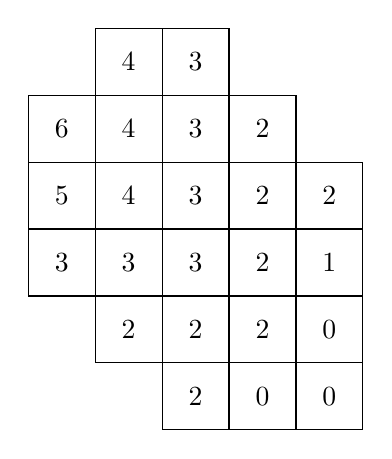
\begin{tikzpicture}[scale=0.85]
  % Helper: draw a cell at (col, row) in English convention (row 0 = top)
  % with label text. Thick edges on the staircase boundary.
  \newcommand{\cell}[3]{% col, row, label
    \fill[white] (#1, -#2) rectangle ++(1,-1);
    \draw (#1, -#2) rectangle ++(1,-1);
    \node at (#1+0.5, -#2-0.5) {$#3$};
  }

  % Row 0 (top): cols 1-2, entries 4, 3
  \cell{1}{0}{4}  \cell{2}{0}{3}
  % Row 1: cols 0-3, entries 6, 4, 3, 2
  \cell{0}{1}{6}  \cell{1}{1}{4}  \cell{2}{1}{3}  \cell{3}{1}{2}
  % Row 2: cols 0-4, entries 5, 4, 3, 2, 2
  \cell{0}{2}{5}  \cell{1}{2}{4}  \cell{2}{2}{3}  \cell{3}{2}{2}  \cell{4}{2}{2}
  % Row 3: cols 0-4, entries 3, 3, 3, 2, 1
  \cell{0}{3}{3}  \cell{1}{3}{3}  \cell{2}{3}{3}  \cell{3}{3}{2}  \cell{4}{3}{1}
  % Row 4: cols 1-4, entries 2, 2, 2, 0
  \cell{1}{4}{2}  \cell{2}{4}{2}  \cell{3}{4}{2}  \cell{4}{4}{0}
  % Row 5: cols 2-4, entries 2, 0, 0
  \cell{2}{5}{2}  \cell{3}{5}{0}  \cell{4}{5}{0}

\end{tikzpicture}
\end{center}





  
  

For a ``cell'' with label k we can imagine k ``cubes'' stacked up on top of the page. Each ``cube'' corresponds to a ``square'' in one of the underlying integer partitions.



  
  \bigskip
\begin{center}
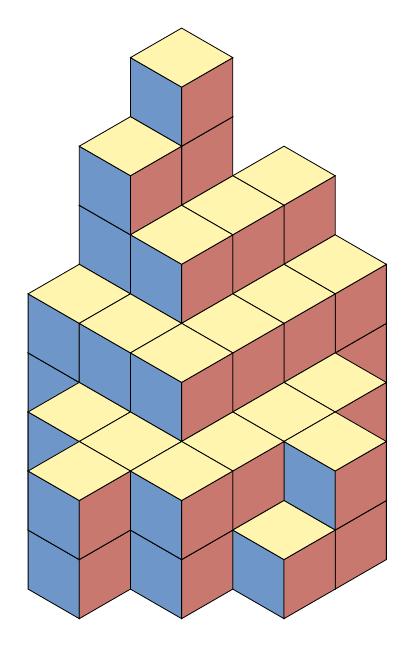
\begin{tikzpicture}[
  % Isometric axes: x = column (lower-right), y = row (lower-left), z = height (up)
  x={(0.65cm, -0.375cm)},
  y={(-0.65cm, -0.375cm)},
  z={(0cm, 0.75cm)}
]

%% Cube face colours
\definecolor{cTop}{RGB}{255,245,175}     % warm yellow
\definecolor{cLeft}{RGB}{110,150,200}    % steel blue
\definecolor{cRight}{RGB}{200,120,110}   % salmon red

%% Macro: draw one unit cube at grid position (c, r, z).
%% Viewer is at (+inf,+inf,+inf), so the THREE VISIBLE faces are:
%%   Top   = z+1 level (horizontal diamond)
%%   Left  = y=r+1 side (left parallelogram on screen)
%%   Right = x=c+1 side (right parallelogram on screen)
%% Draw order: left, right, top (top last covers shared edges cleanly).
\newcommand{\isocube}[3]{%
  % Left face (y=r+1 side, visible from viewer's left)
  \fill[cLeft, draw=black, line width=0.3pt]
    (#1,#2+1,#3) -- (#1+1,#2+1,#3) -- (#1+1,#2+1,#3+1) -- (#1,#2+1,#3+1) -- cycle;
  % Right face (x=c+1 side, visible from viewer's right)
  \fill[cRight, draw=black, line width=0.3pt]
    (#1+1,#2,#3) -- (#1+1,#2+1,#3) -- (#1+1,#2+1,#3+1) -- (#1+1,#2,#3+1) -- cycle;
  % Top face (z+1 level)
  \fill[cTop, draw=black, line width=0.3pt]
    (#1,#2,#3+1) -- (#1+1,#2,#3+1) -- (#1+1,#2+1,#3+1) -- (#1,#2+1,#3+1) -- cycle;
}

%% Draw all cube stacks, sorted by depth c+r (ascending = back to front).
%% Within each depth group, order is irrelevant (no screen overlap).
%% For each position, z iterates 0..h-1 (bottom to top).
%%
%% Data (column, row, height):
%%   Depth 1: (1,0,4), (0,1,6)
%%   Depth 2: (2,0,3), (1,1,4), (0,2,5)
%%   Depth 3: (2,1,3), (1,2,4), (0,3,3)
%%   Depth 4: (3,1,2), (2,2,3), (1,3,3)
%%   Depth 5: (3,2,2), (2,3,3), (1,4,2)
%%   Depth 6: (4,2,2), (3,3,2), (2,4,2)
%%   Depth 7: (4,3,1), (3,4,2), (2,5,2)

\foreach \c/\r/\h in {%
  1/0/4, 0/1/6,%                          depth 1
  2/0/3, 1/1/4, 0/2/5,%                   depth 2
  2/1/3, 1/2/4, 0/3/3,%                   depth 3
  3/1/2, 2/2/3, 1/3/3,%                   depth 4
  3/2/2, 2/3/3, 1/4/2,%                   depth 5
  4/2/2, 3/3/2, 2/4/2,%                   depth 6
  4/3/1, 3/4/2, 2/5/2%                    depth 7
}{%
  \pgfmathtruncatemacro{\maxz}{\h-1}%
  \foreach \z in {0,...,\maxz}{%
    \isocube{\c}{\r}{\z}%
  }%
}

\end{tikzpicture}
\end{center}


\newpage

Each ``square'' in column~$k$ of a Young diagram belongs to \textbf{level~$k$}. These are the ``cubes'' of height $k$. We \textbf{crush} level~$k$ by replacing all labels $k$ with $k-1$.




\bigskip
\begin{center}
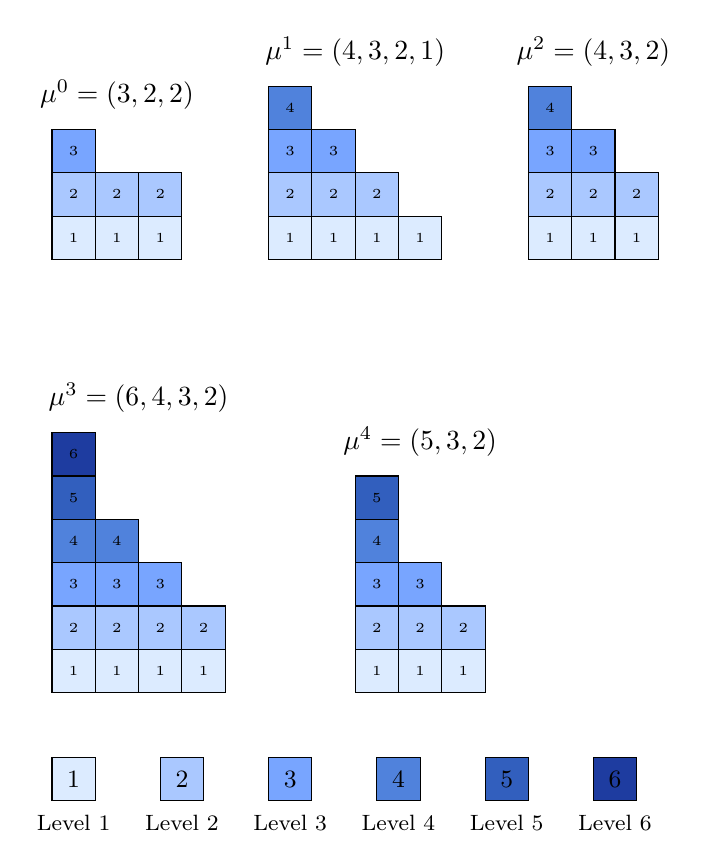
\begin{tikzpicture}[scale=0.55]
  \newcommand{\ringcell}[4]{% x, y (from bottom), col (1-indexed), value
    \pgfmathtruncatemacro{\ringnum}{#3}
    \ifcase\ringnum\or
      \fill[ring1] (#1,#2) rectangle ++(1,1);\or
      \fill[ring2] (#1,#2) rectangle ++(1,1);\or
      \fill[ring3] (#1,#2) rectangle ++(1,1);\or
      \fill[ring4] (#1,#2) rectangle ++(1,1);\or
      \fill[ring5] (#1,#2) rectangle ++(1,1);\or
      \fill[ring6] (#1,#2) rectangle ++(1,1);\fi
    \draw (#1,#2) rectangle ++(1,1);
    \node[font=\tiny] at (#1+0.5,#2+0.5) {#3};
  }
  

  %% Reflected through SW-NE diagonal: rings appear as horizontal layers.
  %% Ring 1 (innermost) at bottom, ring 6 (outermost) at top.

  %% mu^0 = (3,2,2), conjugate = (3,3,1)
  \begin{scope}[xshift=0cm]
    \node at (1.5, 3.8) {$\mu^0 = (3,2,2)$};
    \ringcell{0}{0}{1}{} \ringcell{1}{0}{1}{} \ringcell{2}{0}{1}{}
    \ringcell{0}{1}{2}{} \ringcell{1}{1}{2}{} \ringcell{2}{1}{2}{}
    \ringcell{0}{2}{3}{}
  \end{scope}

  %% mu^1 = (4,3,2,1), conjugate = (4,3,2,1)
  \begin{scope}[xshift=5cm]
    \node at (2, 4.8) {$\mu^1 = (4,3,2,1)$};
    \ringcell{0}{0}{1}{} \ringcell{1}{0}{1}{} \ringcell{2}{0}{1}{} \ringcell{3}{0}{1}{}
    \ringcell{0}{1}{2}{} \ringcell{1}{1}{2}{} \ringcell{2}{1}{2}{}
    \ringcell{0}{2}{3}{} \ringcell{1}{2}{3}{}
    \ringcell{0}{3}{4}{}
  \end{scope}

  %% mu^2 = (4,3,2), conjugate = (3,3,2,1)
  \begin{scope}[xshift=11cm]
    \node at (1.5, 4.8) {$\mu^2 = (4,3,2)$};
    \ringcell{0}{0}{1}{} \ringcell{1}{0}{1}{} \ringcell{2}{0}{1}{}
    \ringcell{0}{1}{2}{} \ringcell{1}{1}{2}{} \ringcell{2}{1}{2}{}
    \ringcell{0}{2}{3}{} \ringcell{1}{2}{3}{}
    \ringcell{0}{3}{4}{}
  \end{scope}

  %% mu^3 = (6,4,3,2), conjugate = (4,4,3,2,1,1)
  \begin{scope}[xshift=0cm, yshift=-10cm]
    \node at (2, 6.8) {$\mu^3 = (6,4,3,2)$};
    \ringcell{0}{0}{1}{} \ringcell{1}{0}{1}{} \ringcell{2}{0}{1}{} \ringcell{3}{0}{1}{}
    \ringcell{0}{1}{2}{} \ringcell{1}{1}{2}{} \ringcell{2}{1}{2}{} \ringcell{3}{1}{2}{}
    \ringcell{0}{2}{3}{} \ringcell{1}{2}{3}{} \ringcell{2}{2}{3}{}
    \ringcell{0}{3}{4}{} \ringcell{1}{3}{4}{}
    \ringcell{0}{4}{5}{}
    \ringcell{0}{5}{6}{}
  \end{scope}

  %% mu^4 = (5,3,2), conjugate = (3,3,2,1,1)
  \begin{scope}[xshift=7cm, yshift=-10cm]
    \node at (1.5, 5.8) {$\mu^4 = (5,3,2)$};
    \ringcell{0}{0}{1}{} \ringcell{1}{0}{1}{} \ringcell{2}{0}{1}{}
    \ringcell{0}{1}{2}{} \ringcell{1}{1}{2}{} \ringcell{2}{1}{2}{}
    \ringcell{0}{2}{3}{} \ringcell{1}{2}{3}{}
    \ringcell{0}{3}{4}{}
    \ringcell{0}{4}{5}{}
  \end{scope}

  %% Legend
  \begin{scope}[xshift=0cm, yshift=-12.5cm]
    \foreach \r/\c/\lab in {1/ring1/1, 2/ring2/2, 3/ring3/3, 4/ring4/4, 5/ring5/5, 6/ring6/6} {
      \pgfmathsetmacro{\xpos}{(\r-1)*2.5}
      \fill[\c] (\xpos,0) rectangle ++(1,1);
      \draw (\xpos,0) rectangle ++(1,1);
      \node at (\xpos+0.5, 0.5) {\small \lab};
      \node[below] at (\xpos+0.5, -0.1) {\footnotesize Level \lab};
    }
  \end{scope}
\end{tikzpicture}
\end{center}




\bigskip
\noindent\textbf{Example: crushing ring 3.}
Six cells in the labelled diagram carry label~3; all become~2.
The resulting partition sequence is:
\[
  \mu^0 = (2,2,2),\quad
  \mu^1 = (4,2,2,1),\quad
  \mu^2 = (4,2,2),\quad
  \mu^3 = (6,4,2,2),\quad
  \mu^4 = (5,2,2).
\]

\medskip
\begin{center}
\renewcommand{\arraystretch}{1.2}
\begin{tabular}{c|c|c|c}
  & \textbf{Before} & \textbf{After} & \textbf{Cells changed} \\ \hline
$\mu^0$ & $(3,2,2)$ & $(2,2,2)$ & 1 \\
$\mu^1$ & $(4,3,2,1)$ & $(4,2,2,1)$ & 1 \\
$\mu^2$ & $(4,3,2)$ & $(4,2,2)$ & 1 \\
$\mu^3$ & $(6,4,3,2)$ & $(6,4,2,2)$ & 1 \\
$\mu^4$ & $(5,3,2)$ & $(5,2,2)$ & 1
\end{tabular}
\end{center}

\newcommand{\pcell}[3]{% col, row, label
  \fill[white] (#1, -#2) rectangle ++(1,-1);
  \draw (#1, -#2) rectangle ++(1,-1);
  \node[font=\small] at (#1+0.5, -#2-0.5) {$#3$};
}

\newpage

\noindent Labelled diagram after crushing level~3:

\smallskip
\begin{center}
\begin{tikzpicture}[scale=0.65]
  \pcell{1}{0}{4}  \pcell{2}{0}{2}
  \pcell{0}{1}{6}  \pcell{1}{1}{4}  \pcell{2}{1}{2}  \pcell{3}{1}{2}
  \pcell{0}{2}{5}  \pcell{1}{2}{4}  \pcell{2}{2}{2}  \pcell{3}{2}{2}  \pcell{4}{2}{2}
  \pcell{0}{3}{2}  \pcell{1}{3}{2}  \pcell{2}{3}{2}  \pcell{3}{3}{2}  \pcell{4}{3}{1}
  \pcell{1}{4}{2}  \pcell{2}{4}{2}  \pcell{3}{4}{2}  \pcell{4}{4}{0}
  \pcell{2}{5}{2}  \pcell{3}{5}{0}  \pcell{4}{5}{0}
\end{tikzpicture}
\end{center}

\noindent 3D isometric view after crushing level~3:

\bigskip
\begin{center}
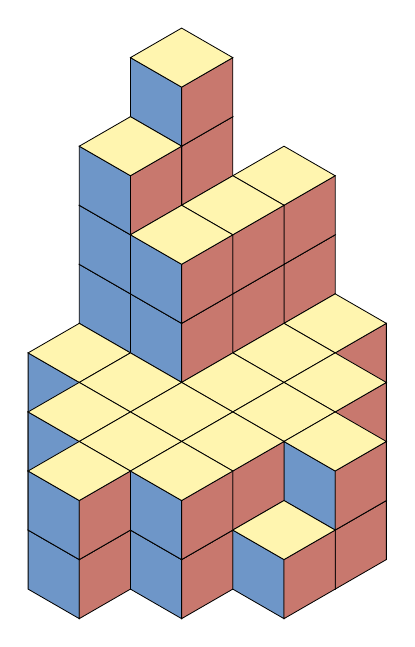
\begin{tikzpicture}[
  x={(0.65cm, -0.375cm)},
  y={(-0.65cm, -0.375cm)},
  z={(0cm, 0.75cm)}
]

\definecolor{cTop}{RGB}{255,245,175}
\definecolor{cLeft}{RGB}{110,150,200}
\definecolor{cRight}{RGB}{200,120,110}

\newcommand{\crushedcube}[3]{%
  \fill[cLeft, draw=black, line width=0.3pt]
    (#1,#2+1,#3) -- (#1+1,#2+1,#3) -- (#1+1,#2+1,#3+1) -- (#1,#2+1,#3+1) -- cycle;
  \fill[cRight, draw=black, line width=0.3pt]
    (#1+1,#2,#3) -- (#1+1,#2+1,#3) -- (#1+1,#2+1,#3+1) -- (#1+1,#2,#3+1) -- cycle;
  \fill[cTop, draw=black, line width=0.3pt]
    (#1,#2,#3+1) -- (#1+1,#2,#3+1) -- (#1+1,#2+1,#3+1) -- (#1,#2+1,#3+1) -- cycle;
}

%% Height data after crushing ring 3, sorted by depth c+r.
\foreach \c/\r/\h in {%
  1/0/4, 0/1/6,%                          depth 1
  2/0/2, 1/1/4, 0/2/5,%                   depth 2
  2/1/2, 1/2/4, 0/3/2,%                   depth 3
  3/1/2, 2/2/2, 1/3/2,%                   depth 4
  3/2/2, 2/3/2, 1/4/2,%                   depth 5
  4/2/2, 3/3/2, 2/4/2,%                   depth 6
  4/3/1, 3/4/2, 2/5/2%                    depth 7
}{%
  \pgfmathtruncatemacro{\maxz}{\h-1}%
  \foreach \z in {0,...,\maxz}{%
    \crushedcube{\c}{\r}{\z}%
  }%
}

\end{tikzpicture}
\end{center}

\newpage

\noindent Another way to represent cylindric plane partitions is with non-intersecting lattice paths on a cylinder.

\bigskip
\begin{center}
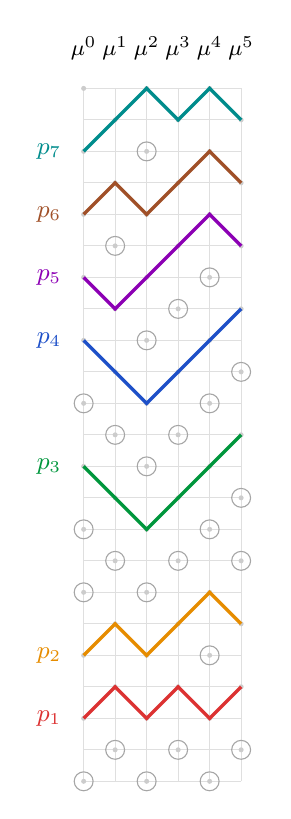
\begin{tikzpicture}[scale=0.8]

  %% Path colours (7 paths = weight of base partition |mu^0| = 3+2+2 = 7)
  \definecolor{p1col}{RGB}{220,50,50}     % red
  \definecolor{p2col}{RGB}{230,140,0}     % orange
  \definecolor{p3col}{RGB}{0,150,60}      % green
  \definecolor{p4col}{RGB}{30,80,200}     % blue
  \definecolor{p5col}{RGB}{140,0,180}     % purple
  \definecolor{p6col}{RGB}{160,80,40}     % brown
  \definecolor{p7col}{RGB}{0,140,140}     % teal

  %% Grid background
  \draw[step=0.5cm, gray!25] (0,0) grid (2.5,11);

  %% Lattice dots (integer grid: y = 0,...,11)
  \foreach \i in {0,...,2} {
    \foreach \j in {0,...,11} {
      \fill[gray!40] (\i,\j) circle (0.4mm);
    }
  }
  %% Lattice dots (half-integer grid: y = 0.5,...,10.5)
  \foreach \i in {0,...,2} {
    \foreach \j in {0,...,10} {
      \fill[gray!40] (\i+0.5,\j+0.5) circle (0.4mm);
    }
  }

  %% Vacancy markers (Maya diagram holes) — open circles
  %% x=0 (mu^0 = (3,2,2)): vacancies at y = 0, 3, 4, 6
  \foreach \y in {0,3,4,6} { \draw[gray!70] (0,\y) circle (1.5mm); }
  %% x=0.5 (mu^1 = (4,3,2,1)): vacancies at y = 0.5, 3.5, 5.5, 8.5
  \foreach \y in {0.5,3.5,5.5,8.5} { \draw[gray!70] (0.5,\y) circle (1.5mm); }
  %% x=1 (mu^2 = (4,3,2)): vacancies at y = 0, 3, 5, 7, 10
  \foreach \y in {0,3,5,7,10} { \draw[gray!70] (1,\y) circle (1.5mm); }
  %% x=1.5 (mu^3 = (6,4,3,2)): vacancies at y = 0.5, 3.5, 5.5, 7.5
  \foreach \y in {0.5,3.5,5.5,7.5} { \draw[gray!70] (1.5,\y) circle (1.5mm); }
  %% x=2 (mu^4 = (5,3,2)): vacancies at y = 0, 2, 4, 6, 8
  \foreach \y in {0,2,4,6,8} { \draw[gray!70] (2,\y) circle (1.5mm); }
  %% x=2.5 (mu^5 = (3,2,2)): vacancies at y = 0.5, 3.5, 4.5, 6.5
  \foreach \y in {0.5,3.5,4.5,6.5} { \draw[gray!70] (2.5,\y) circle (1.5mm); }

  %% 7 non-intersecting lattice paths
  \draw[very thick, p1col]
    (0,1) -- (0.5,1.5) -- (1,1) -- (1.5,1.5) -- (2,1) -- (2.5,1.5);
  \draw[very thick, p2col]
    (0,2) -- (0.5,2.5) -- (1,2) -- (1.5,2.5) -- (2,3) -- (2.5,2.5);
  \draw[very thick, p3col]
    (0,5) -- (0.5,4.5) -- (1,4) -- (1.5,4.5) -- (2,5) -- (2.5,5.5);
  \draw[very thick, p4col]
    (0,7) -- (0.5,6.5) -- (1,6) -- (1.5,6.5) -- (2,7) -- (2.5,7.5);
  \draw[very thick, p5col]
    (0,8) -- (0.5,7.5) -- (1,8) -- (1.5,8.5) -- (2,9) -- (2.5,8.5);
  \draw[very thick, p6col]
    (0,9) -- (0.5,9.5) -- (1,9) -- (1.5,9.5) -- (2,10) -- (2.5,9.5);
  \draw[very thick, p7col]
    (0,10) -- (0.5,10.5) -- (1,11) -- (1.5,10.5) -- (2,11) -- (2.5,10.5);

  %% Path labels (left side)
  \node[left, p1col, font=\small\bfseries] at (-0.2,1) {$p_1$};
  \node[left, p2col, font=\small\bfseries] at (-0.2,2) {$p_2$};
  \node[left, p3col, font=\small\bfseries] at (-0.2,5) {$p_3$};
  \node[left, p4col, font=\small\bfseries] at (-0.2,7) {$p_4$};
  \node[left, p5col, font=\small\bfseries] at (-0.2,8) {$p_5$};
  \node[left, p6col, font=\small\bfseries] at (-0.2,9) {$p_6$};
  \node[left, p7col, font=\small\bfseries] at (-0.2,10) {$p_7$};

  %% Column partition labels (above)
  \node[above, font=\footnotesize] at (0,11.3) {$\mu^0$};
  \node[above, font=\footnotesize] at (0.5,11.3) {$\mu^1$};
  \node[above, font=\footnotesize] at (1,11.3) {$\mu^2$};
  \node[above, font=\footnotesize] at (1.5,11.3) {$\mu^3$};
  \node[above, font=\footnotesize] at (2,11.3) {$\mu^4$};
  \node[above, font=\footnotesize] at (2.5,11.3) {$\mu^5$};

\end{tikzpicture}
\end{center}


This construction uses the natural bijection between integer partitions and binary strings.
The profile $\pi = 1001010100$ encodes the partition $\gamma = (6,4,3,2)$
via the boundary path of the Young diagram inside a $6 \times 4$ rectangle.
Reading $\pi$ left to right: $1$ = down step, $0$ = horizontal step.

\bigskip
\begin{center}
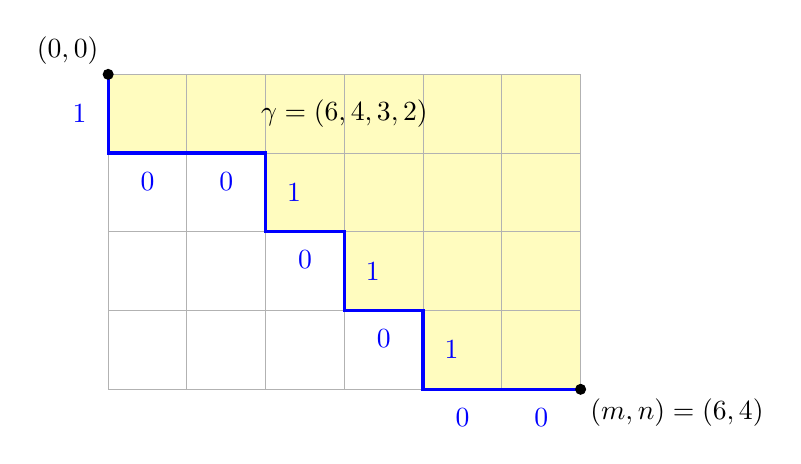
\begin{tikzpicture}[scale=1.0]

  %% Grid
  \draw[gray!40] (0,0) grid (6,4);

  %% Partition cells (shaded) — English convention (widest row at top)
  \fill[yellow!25] (0,3) rectangle (6,4);  % row 1: 6 cells (top)
  \fill[yellow!25] (2,2) rectangle (6,4);  % row 2: 4 cells
  \fill[yellow!25] (3,1) rectangle (6,4);  % row 3: 3 cells
  \fill[yellow!25] (4,0) rectangle (6,4);  % row 4: 2 cells (bottom)

  %% Redraw grid on top
  \draw[gray!60] (0,0) grid (6,4);

  %% Boundary path (thick blue) — flipped vertically (y -> 4-y)
  %% pi = 1,0,0,1,0,1,0,1,0,0
  %% (0,4)->(0,3)->(1,3)->(2,3)->(2,2)->(3,2)->(3,1)->(4,1)->(4,0)->(5,0)->(6,0)
  \draw[very thick, blue]
    (0,4) -- (0,3) -- (1,3) -- (2,3) -- (2,2) -- (3,2) -- (3,1) -- (4,1) -- (4,0) -- (5,0) -- (6,0);

  %% Step labels: 1 0 0 1 0 1 0 1 0 0
  %% Vertical "1" labels on the right; horizontal "0" labels below.
  \node[left, blue, font=\bfseries] at (-0.15, 3.5) {$1$};
  \node[below, blue, font=\bfseries] at (0.5, 2.88) {$0$};
  \node[below, blue, font=\bfseries] at (1.5, 2.88) {$0$};
  \node[right, blue, font=\bfseries] at (2.15, 2.5) {$1$};
  \node[below, blue, font=\bfseries] at (2.5, 1.88) {$0$};
  \node[right, blue, font=\bfseries] at (3.15, 1.5) {$1$};
  \node[below, blue, font=\bfseries] at (3.5, 0.88) {$0$};
  \node[right, blue, font=\bfseries] at (4.15, 0.5) {$1$};
  \node[below, blue, font=\bfseries] at (4.5, -0.12) {$0$};
  \node[below, blue, font=\bfseries] at (5.5, -0.12) {$0$};

  %% Start/end dots
  \fill (0,4) circle (2pt);
  \fill (6,0) circle (2pt);

  %% Corner labels
  \node[above left] at (0,4) {$(0,0)$};
  \node[below right] at (6,0) {$(m,n) = (6,4)$};

  %% Partition label
  \node at (3, 3.5) {$\gamma = (6,4,3,2)$};

\end{tikzpicture}
\end{center}

Crushing level $k$ of a family of non-intersecting lattice paths is equivalent to pushing the $k$th path flush up against the one above it. 

\newpage

The formula for the enumeration of Cylindric Plane Partitions was originally given by Borodin:

\begin{equation} \label{borodin}
\sum_{\mathfrak{c} \in \CPP(\pi)} z^{|\mathfrak{c}|} = 
\prod_{n \geq 0} \left ( \frac{1}{1-z^{(n+1)T}} \prod_{\substack{i < j \\ \pi_i > \pi_j}} \frac{1}{1-z^{j-i + nT}} 
\prod_{\substack{i > j \\ \pi_i > \pi_j }} \frac{1}{1 - z^{j-i + (n+1)T}} \right ) 
\end{equation}

In my thesis I proved this result using growth diagrams:


\begin{center}
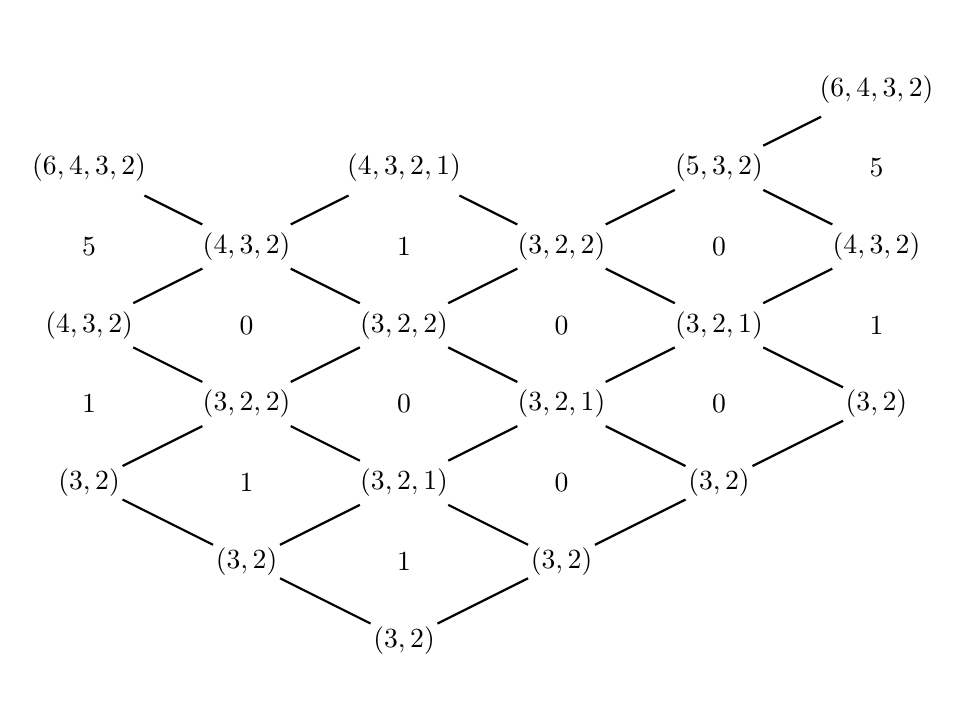
\begin{tikzpicture}[scale=1]

\begin{scope}
\path (-4,2) node[shape=circle,inner sep=0.3mm](A0){$(3,2)$};
\path (-2,1) node[shape=circle,inner sep=0.3mm](B0){$(3,2)$};
\path (0,0) node[shape=circle,inner sep=0.3mm](C0){$(3,2)$};
\path (2,1) node[shape=circle,inner sep=0.3mm](D0){$(3,2)$};
\path (4,2) node[shape=circle,inner sep=0.3mm](E0){$(3,2)$};
\path (6,3) node[shape=circle,inner sep=0.3mm](F0){$(3,2)$};

\path (-4,4) node[shape=circle,inner sep=0.3mm](A1){$(4,3,2)$};
\path (-2,3) node[shape=circle,inner sep=0.3mm](B1){$(3,2,2)$};
\path (0,2) node[shape=circle,inner sep=0.3mm](C1){$(3,2,1)$};
\path (2,3) node[shape=circle,inner sep=0.3mm](D1){$(3,2,1)$};
\path (4,4) node[shape=circle,inner sep=0.3mm](E1){$(3,2,1)$};
\path (6,5) node[shape=circle,inner sep=0.3mm](F1){$(4,3,2)$};

\path (-4,6) node[shape=circle,inner sep=0.3mm](A2){$(6,4,3,2)$};
\path (-2,5) node[shape=circle,inner sep=0.3mm](B2){$(4,3,2)$};
\path (0,4) node[shape=circle,inner sep=0.3mm](C2){$(3,2,2)$};
\path (2,5) node[shape=circle,inner sep=0.3mm](D2){$(3,2,2)$};
\path (4,6) node[shape=circle,inner sep=0.3mm](E2){$(5,3,2)$};
\path (6,7) node[shape=circle,inner sep=0.3mm](F2){$(6,4,3,2)$};

\path (0,6) node[shape=circle,inner sep=0.3mm](C3){$(4,3,2,1)$};

\draw[thick] (A0) -- (B0) -- (C0) -- (D0) -- (E0) -- (F0);
\draw[thick] (A1) -- (B1) -- (C1) -- (D1) -- (E1) -- (F1);
\draw[thick] (A2) -- (B2) -- (C2) -- (D2) -- (E2) -- (F2);

\draw[thick] (A1) -- (B2) -- (C3);
\draw[thick] (A0) -- (B1) -- (C2);
\draw[thick] (B0) -- (C1);
\draw[thick] (D0) -- (C1);
\draw[thick] (E0) -- (D1) -- (C2);
\draw[thick] (F0) -- (E1) -- (D2) -- (C3);
\draw[thick] (F1) -- (E2);

\path (-4,3) node[shape=circle,inner sep=0.3mm](a0){$1$};
\path (-2,2) node[shape=circle,inner sep=0.3mm](b0){$1$};
\path (0,1) node[shape=circle,inner sep=0.3mm](c0){$1$};
\path (2,2) node[shape=circle,inner sep=0.3mm](dD0){$0$};
\path (4,3) node[shape=circle,inner sep=0.3mm](e0){$0$};
\path (6,4) node[shape=circle,inner sep=0.3mm](f0){$1$};

\path (-4,5) node[shape=circle,inner sep=0.3mm](a1){$5$};
\path (-2,4) node[shape=circle,inner sep=0.3mm](b1){$0$};
\path (0,3) node[shape=circle,inner sep=0.3mm](c1){$0$};
\path (2,4) node[shape=circle,inner sep=0.3mm](d1){$0$};
\path (4,5) node[shape=circle,inner sep=0.3mm](e1){$0$};
\path (6,6) node[shape=circle,inner sep=0.3mm](f1){$5$};

\path (0,5) node[shape=circle,inner sep=0.3mm](v2){$1$};
\end{scope}

\end{tikzpicture}
\end{center}

The right hand side of the equation can be interpreted as a pair $(\gamma, \mathfrak{d})$ where $\gamma$ is an integer partition and $\mathfrak{d}$ is a ``hook length weighted labelled cylindric diagram''. The proof makes use of ``local rules''. To understand the local rules we need to look at Cauchy's Identity.

\newpageß

\begin{proposition}
If $X_n$ is the alphabet $X_n = x_1 + x_2 + \cdots + x_n$
and $Y_n$ is the alphabet $Y_n = y_1 + y_2 + \cdots + y_n$ then:
\[ \sum_\lambda S_\lambda[X_n] S_\lambda[Y_n] = \prod_{i,j=1}^n \frac{1}{1-x_iy_j} \]
\begin{proof}
The case $n=1$ is trivial.
We assume that the result is true for all $k < n$.
By the Pieri formula and the induction assumption, we have on the right hand side:

\begin{align*}
RHS(n) & = \left (\sum_r h_r[X_{n-1}] x_n^r \right ) 
\left (\sum_s h_s[Y_{n-1}] y_n^s \right ) \left (  \sum_\mu S_\mu[X_{n-1}] S_\mu[Y_{n-1}] \right )\frac{1}{1-x_n y_n} \\
& = \sum_{\alpha, \beta} S_{\alpha}[X_{n-1}] S_{\beta}[Y_{n-1}] \left ( \frac{1}{1-x_n y_n} \sum_{\mu \in D(\alpha) \cap D(\beta)} x_n^{|\alpha / \mu|} y_n^{|\beta / \mu|} \right )
\end{align*}

while by the dual Pieri formula we have on the left hand side:

\begin{align*}
LHS(n) & = \sum_\lambda S_\lambda[X_{n-1} + x_n] S_\lambda[X_{n-1} + y_n] \\
& = \sum_{\alpha, \beta} S_\alpha[X_{n-1}] S_\beta[Y_{n-1}] \left ( \sum_{\lambda \in U(\alpha) \cap U(\beta)} x_n^{|\lambda / \alpha|} y_n^{|\lambda / \beta|} \right )
\end{align*}


In order to complete this proof, we need, for any given $\alpha$ and $\beta$ a bijection between the set of pairs $(m,\mu)$ with $\mu \in D(\alpha) \cup D(\beta)$ and $m$ a non-negative integer and the set of partitions $\lambda \in U(\alpha) \cup U(\beta)$ in such a way that:
\[ |\lambda|  = |\alpha | + |\beta| - |\mu| + m \]
A \emph{local rule}  is just such a bijection. 
\begin{equation}
\mathfrak{U}_{\alpha,\beta} : (\mathbb{Z}_{\geq 0}, D(\alpha) \cup D(\beta)) \to U(\alpha) \cup U(\beta)
\end{equation}

\end{proof}
\end{proposition}

\newpage

\begin{definition}
Consider the graded generating series for cylindric play partitions with profile $c$:

\begin{equation}\label{eq:gm}
  \GK_c(z,q) = \sum_m g_m(q) z^m 
  = \sum_{\pi \in \CPP(c)}
    q^{|\pi|}z^{\max(\pi)}.
\end{equation}


The \emph{$Q$-polynomial} is defined by:
\begin{equation}\label{eq:Q-def}
  Q_{n,c}(q)
  = \qpochn{q}{q}{n}
    \cdot [z^n]\bigl(\qpoch{zq}{q} \cdot \GK_c(z,q)\bigr).
\end{equation}
\end{definition}

\begin{conjecture}[Warnaar--Corteel]
\label{conj:main}
For all $n \geq 0$ and all rank-$3$ profiles~$c$,
\[
  Q_{n,c}(q) \in \N[q].
\]
\end{conjecture}


\begin{proposition}
If $g_m(q) = \sum_n \mathcal{G}_{n,c} q^n$ then with some straightforeward manipulation we can show that:

\begin{equation}\label{eq:G-triples}
  \widetilde{\mathcal{G}}_{n,c} =
  \bigsqcup_{j=0}^{n}
  \left\{(S, U, \nu) :
    \begin{array}{l}
      S \subseteq \{1,\ldots,n\},\; |S| = j, \\[2pt]
      U \subseteq \{1,\ldots,n-j\}, \\[2pt]
      \nu \in \CPP(c),\; \max(\nu) = n - j
    \end{array}
  \right\},
\end{equation}
with sign $\varepsilon(S, U, \nu) = (-1)^{|S| + |U|}$ and weight
$w(S, U, \nu) = \sigma(S) + \sigma(U) + |\nu|$.
\begin{proof}
We expand the three factors in~\eqref{eq:Q-def}.

\medskip\noindent\textbf{Step 1: Euler's identity.}
The $q$-Pochhammer product has the expansion
\[
  \qpoch{zq}{q} = \sum_{j \geq 0} \frac{(-1)^j\, q^{j(j+1)/2}}{\qpochn{q}{q}{j}}\, z^j.
\]

\medskip\noindent\textbf{Step 2: Extract the $z^n$ coefficient.}
Multiplying by $\GK_c(z,q) = \sum_m g_m(q)\, z^m$ and extracting $[z^n]$:
\[
  [z^n]\bigl(\qpoch{zq}{q} \cdot \GK_c(z,q)\bigr)
  = \sum_{j=0}^{n} \frac{(-1)^j\, q^{j(j+1)/2}}{\qpochn{q}{q}{j}}\, g_{n-j}(q).
\]
Multiplying by $\qpochn{q}{q}{n}$ and using
$\frac{\qpochn{q}{q}{n}}{\qpochn{q}{q}{j}} = \qbin{n}{j}\,\qpochn{q}{q}{n-j}$:
\begin{equation}\label{eq:Q-expand}
  Q_{n,c}(q) = \sum_{j=0}^{n} (-1)^j\, q^{j(j+1)/2}\, \qbin{n}{j}\, \qpochn{q}{q}{n-j}\, g_{n-j}(q).
\end{equation}

\medskip\noindent\textbf{Step 3: Combinatorial interpretation of each factor.}

Recall that the \emph{$q$-binomial coefficient} counts partitions fitting inside a $j \times (n{-}j)$ rectangle:
\[
  \qbin{n}{j} := \frac{\qpochn{q}{q}{n}}{\qpochn{q}{q}{j}\,\qpochn{q}{q}{n-j}} = \sum_{\lambda \subseteq (n-j)^j} q^{|\lambda|}.
\]
One can show that for integers $0 \leq j \leq n$,
\begin{equation}\label{eq:qbin-subsets}
  q^{j(j+1)/2}\,\qbin{n}{j}
  = \sum_{\substack{S \subseteq \{1,\ldots,n\} \\ |S| = j}} q^{\sigma(S)},
\end{equation}
where $\sigma(S) = \sum_{s \in S} s$.
Similarly, the finite $q$-Pochhammer symbol expands as:
\begin{equation}\label{eq:qpoch-subsets}
  \qpochn{q}{q}{m} = \prod_{k=1}^{m}(1-q^k) = \sum_{U \subseteq \{1,\ldots,m\}} (-1)^{|U|}\, q^{\sigma(U)}.
\end{equation}
Finally, $g_m(q) = \sum_{\nu \in \CPP(c),\, \max(\nu)=m} q^{|\nu|}$ by definition of~$\GK_c$.

\medskip\noindent\textbf{Step 4: Combine.}
Substituting \eqref{eq:qbin-subsets}, \eqref{eq:qpoch-subsets}, and the definition of~$g_m$ into~\eqref{eq:Q-expand} with $m = n - j$:
\[
  Q_{n,c}(q) = \sum_{j=0}^{n}\;
  \sum_{\substack{S \subseteq \{1,\ldots,n\} \\ |S|=j}}\;
  \sum_{U \subseteq \{1,\ldots,n-j\}}\;
  \sum_{\substack{\nu \in \CPP(c) \\ \max(\nu) = n-j}}
  (-1)^{|S|+|U|}\, q^{\sigma(S)+\sigma(U)+|\nu|}.
\]
Since $j = |S|$, this is precisely the signed generating function over the ground set~$\widetilde{\mathcal{G}}_{n,c}$.
\end{proof}
\end{proposition}

\newpage

\section{Multi-variate analog}

We replace $q^k$ with $q_k$ and when $c$ is a cylindric plane partition we replace $q^c$ with 
$q_{\lambda_1} q_{\lambda_2}  q_{\lambda_3}$. The definition of $Q_n(q_1, q_2, ....) $ becomes:


\begin{eqnarray} Q_n(q_1, q_2....) & = \sum_k (-1)^k e_k(q_1, q_2, ....) [z^n] \sum_k (-1)^k e_k(q_1,q_2,....) 
\sum_c q_{\lambda_1} q_{\lambda_2} q_{\lambda_3} z^{max(c)} \\
& =
\end{eqnarray}

Does the right hand side look like this:

\[ \sum (S,U, \nu) (\prod_{s \in S} \prod_{u \in u} q_s q_u) \sum q_{\lambda_1} q_{\lambda_2} q_{\lambda_3} \]] 


\newpage

Start with a cylindric plane partition $\lambda$ with maximum entry $n$. This corresponds to a family of $n+1$ non-intersecting lattice paths. The set S is of size j. So we remove j paths (not including the top one), corresponding to the elements of S. This leaves a partition $\gamma$ with maximum entry $n-j$. Now we have $U$. This set contains $n-j$ elements. Of the remaining paths (excluding the top one) we ``crush'' those corresponding to the elements of $U$. That is we push them up flush against the path immediately above. This gives us a new partition $mu$ also with maximum part $n-j$. This process cannot be revursed. It defines an ``equivalence relation'' on the set of all cylindric plane partitions with maximum part $n$.



\end{document}
